%%%%%%%%%%%%%%%%%%%%%%%%%%%%%%%%%%%%%%%%%%%%%%%%%%%%%%%%%%%%%%%%%%%%%%%%%%%%%%%%
%% An attempt to replicate CAIA Techincal Report Template                     %%
%%%%%%%%%%%%%%%%%%%%%%%%%%%%%%%%%%%%%%%%%%%%%%%%%%%%%%%%%%%%%%%%%%%%%%%%%%%%%%%%

\documentclass[a4paper,twocolumn,english,11pt, a4paper, conference]{IEEEtran}
\IEEEoverridecommandlockouts % So we can use \thanks in the Author list for Isaac's internship note

\usepackage{url}
\usepackage{graphicx}
\usepackage{verbatim}
\usepackage{multicol}
\usepackage{multirow}
\usepackage{amsmath}
\usepackage{inconsolata}
\usepackage{listings}
\usepackage{setspace}
\usepackage{pbox}
\usepackage{booktabs}
%\usepackage{hyperref}
\usepackage[utf8]{inputenc}
\usepackage[T1]{fontenc}
\usepackage{tikz}
\usepackage{pgf-umlsd}
\usepackage{fancyhdr}
\pagestyle{fancy}

\makeatletter


\usepackage{changepage}

\usepackage{lastpage}

% Change the \footnoterule command to separate footnotes from 
% the main text by a short horizontal rule (borrowed
% from the CAIA style)
\renewcommand{\footnoterule}
{
	\kern-3\p@
	\hrule\@width.4\columnwidth
	\kern2.6\p@
}

%% Mimic CAIA TR use of hyperlinks

% The "xcolor" package allows us to define the colours we will use for links   %
% within the PDF when we later load the "hyperref" package.                    %

\RequirePackage{xcolor}
\xdefinecolor{linkc}{RGB}{33,0,99}
\xdefinecolor{citec}{RGB}{0,0,0}
\xdefinecolor{caiablack}{RGB}{0,0,0}
\xdefinecolor{urlc}{RGB}{33,0,99}

% The "hyperref" package allows us to generate a PDF with associated PDF links %
% and bookmarks and other funky PDF stuff.                                     %

\RequirePackage[colorlinks=true,                  % Links are marked as coloured text, not coloured box.
                linkcolor= linkc,                 % Colour of in-document links (e.g. in the table of contents).
                citecolor= caiablack,             % Colour of bibliographic citations.
                urlcolor= urlc,                   % Colour of hyperlinks to the Net.
                pdfpagelayout=SinglePage,         % Initial view is page-by-page
                pdfstartview=FitV,                % Fit the document to window height.
               ]{hyperref}
               
               
\usetikzlibrary{arrows,automata,positioning,shapes,decorations.pathreplacing}


\title{ Teaplot v0.1: A browser-based 3D engine for animating TEACUP experiment data}
\lstset{ basicstyle=\footnotesize\ttfamily,}

\author{\IEEEauthorblockN{Isaac True\IEEEauthorrefmark{1}\thanks{\IEEEauthorrefmark{1}The work described in this report was done during the author's winter internship at CAIA in 2015}, Grenville Armitage, Philip Branch}
\IEEEauthorblockA{Centre for Advanced Internet Architectures\\
Swinburne University of Technology\\
Melbourne, Australia\\
\url{itrue@swin.edu.au}, \url{garmitage@swin.edu.au}, \url{pbranch@swin.edu.au}}}

% \CAIATRAddAuthor{Isaac True}{itrue@swin.edu.au}{The work described in this report was done during the author's winter internship at CAIA in 2015}
% \CAIATRAddAuthor{Grenville Armitage}{garmitage@swin.edu.au}{}
% \CAIATRAddAuthor{Philip Branch}{pbranch@swin.edu.au}{}
% \CAIATRSetDetails{15}{08}{August}{28A}

\newcommand{\sh}[2]{{\small \texttt{#1 #2}}}

%%%%%%%%%%%%%%%%%%%%%%%%%%%%%%%%%%%%%%%%%%%%%%%%%%%%%%%%%%%%%%%%%%%%%%%%%%%%%%%%
%% DOCUMENT BEGINS HERE                                                       %%
%%%%%%%%%%%%%%%%%%%%%%%%%%%%%%%%%%%%%%%%%%%%%%%%%%%%%%%%%%%%%%%%%%%%%%%%%%%%%%%%
\begin{document}

%%%%%%%%%%
% Required to support advanced referencing
%%%%%%%%%%
\bstctlcite{caia-ref}

%%%%%%%%%%
% Make the Title block
%%%%%%%%%%
\maketitle

%%%%%%%%%%
% Define headers and footers to capture CC-BY-SA information
%%%%%%%%%%
\fancypagestyle{firstpage}{% Page style for first page
  \fancyhf{}% Clear header/footer
  \renewcommand{\headrulewidth}{0pt}% Header rule
  \renewcommand{\footrulewidth}{0pt}% Footer rule
  \fancyfoot[C]{\small{\copyright~2015 -- 2016 CAIA, Swinburne University of Technology\\Originally published as \url{http://caia.swin.edu.au/reports/150828A/CAIA-TR-150828A.pdf}\\This version released July 1st 2016 under Creative Commons BY-SA 4.0 License -- see terms on page~\pageref{sec:Copying}}}
}
\thispagestyle{firstpage}
  \pagestyle{fancy}
  \headheight 13.4pt
  \renewcommand{\headrulewidth}{0pt}
  \lfoot{\small{Teaplot v0.1: A browser-based 3D engine for animating TEACUP experiment data}}
  \cfoot{}
  \rfoot{\small{July 1, 2016~~page \thepage ~of \pageref{LastPage}}} 

%%%%%%%%%%
% Modify your document below...
%%%%%%%%%%
\begin{abstract}

TEACUP is a software tool developed at CAIA for running automated TCP experiments, which can generate static PDF graphs of experiment results using R. Teaplot v0.1 is an extension to this tool which allows the user to interactively visualise and animate these results in a web browser in both 2-and 3D. 

This report contains information pertaining to the architecture and technical requirements of the extension, along with the installation procedure and a user interface guide for the web client component.

Ideas for potential further work on Teaplot were identified during development, including bug fixes and solutions for performance and visual issues, and have been included within this report.

\end{abstract}

%\tableofcontents
\section{Introduction}
TEACUP \cite{teacup} is a software tool developed at CAIA for running automated TCP experiments and modelling complex network characteristics and performance in a testbed.  Teaplot v0.1 is an extension to this tool.

Traditionally, TEACUP experiment data is analysed and plotted using scripts written in R \cite{R}, which generate static graphs as PDFs. Changing how the data is displayed means modifying command line arguments and regenerating these graphs, repeatedly -- a time-consuming and repetitive job. Teaplot reinvents this process by providing the user with a graphical interface in their browser which can be used to plot experiment data dynamically, allowing the user to pick and choose results from various experiments, combine multiple measured and calculated metrics, and animate the data as it changes over time across multiple graphs, in both 2- and 3D. 

The current TEACUP version as of the time of writing is v1.0. Further information relating to TEACUP, its operation, and example scenarios for testbeds can be found in the TEACUP technical reports \cite{CAIA-TR-150529A} \cite{CAIA-TR-150529B} \cite{CAIA-TR-150529C} \cite{CAIA-TR-150210C}.

This report is intended to give the reader a technical overview of the functions, requirements, and usage of Teaplot. Section \ref{sect:architecture} details how the system is structured, while Section \ref{sect:requirements} details the technical requirements and software dependencies. Section \ref{sect:installation} describes how to install Teaplot using TEACUP v1.0 as a base. Section \ref{sect:usage} guides the potential user in the use of the client web interface component of Teaplot, and Section \ref{sect:future} gives examples for potential further work that have been identified as useful or beneficial to the performance of the program.
\section{Architecture}
\label{sect:architecture}
\subsection{System Design}
The Teaplot system is separated into two components: the client, and the server. The client component is an HTML5-compliant WebGL-based web page which is used as the user interface for Teaplot, while the server component, written in Python, is responsible for the mathematical and data processing tasks required in creating the data for the animations. All intensive mathematical calculations are performed by the server, where the operations can be accelerated through the use of mathematical libraries such as SciPy and NumPy, which provide Python wrappers around native libraries. The server is also responsible for communicating with TEACUP, in order to extract and utilise the data it makes available. This architecture can be seen in Figure \ref{fig:architecture}.

The server makes available to the client an API, through which the client can request a list of experiments, metrics, and flows, and also request a set of data to be generated for a particular experiment, metric, and flow combination in order to plot and animate it on screen. This design ensures separation of the client and server logic, and facilitates the use of the server-side mathematical libraries as described above. 

The server also provides the HTTP server for the static web pages comprising the client; to use Teaplot, a user simply navigates to the URL of the server using a compatible web browser.

The Teaplot server is implemented as a Fabric \cite{fabric} task called \texttt{animate}, and so easily integrates into existing TEACUP installations. The \texttt{animate} task is easily executed as an argument to the \texttt{fab} task. Details regarding this usage can be found in Section \ref{sect:usage}.
\begin{figure}
	\sffamily
	\small
	\centering
	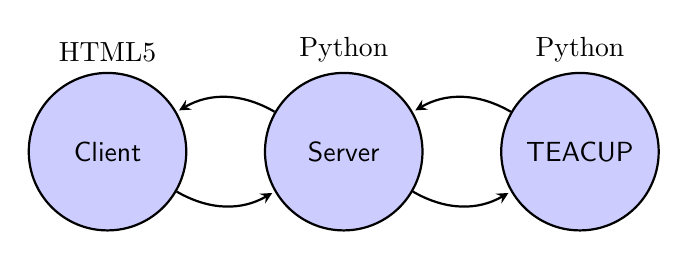
\begin{tikzpicture}[->,>=stealth,shorten >=1pt,auto,node distance=3cm,
	thick,main node/.style={circle,fill=blue!20,draw,font=\sffamily}]
	\node[main node,label={Python},minimum size=2cm] (1) {Server};
	\node[main node,label={HTML5},minimum size=2cm] (2) [left of=1] {Client};
	\node[main node,label={Python},minimum size=2cm] (3) [right of=1] {TEACUP};
	
	\path[every node/.style={font=\sffamily\small}]
	(1) edge [bend right] node [] {} (2)
	edge [bend right] node [] {} (3)
	(2) edge [bend right] node [] {} (1)
	(3) edge [bend right] node [] {} (1);
	\end{tikzpicture}
	\caption{System Architecture Diagram}
	\label{fig:architecture}
\end{figure}
\subsection{API}
The Teaplot server API utilises JSON (JavaScript Object Notation) \cite{json} formatted documents for communicating data. 

Table \ref{table:endpoints} shows a list of endpoints present in the API, which the client application can make use of, and can be used for debugging, if need be.

As the server program is assumed to be short-lived and in a controlled environment, no authentication takes place on the API.

\begin{table}
\centering
\caption{API Endpoints}
\label{table:endpoints}
\begin{tabular}{l c p{4cm}}
	\textbf{ Endpoint} & \textbf{ Type} & \textbf{ Description} \\ \toprule
	\texttt{/api/default} & \texttt{GET} & Default parameters for the client (exp\_id, metric, etc.) \\ \midrule
	\texttt{/api/metrics} &\texttt{GET} & Lists the available metrics, including SIFTR and Web10G metrics if enabled \\ \midrule
	\texttt{/api/metrics/get} & \texttt{POST} & Starts the extraction process for the experiment and metric combination sent as POST data and returns the available data \\ \midrule
	\texttt{/api/experiments} & \texttt{GET} & Lists the available experiments \\ \midrule
	\texttt{/api/graph} & \texttt{POST} & Generates plottable data points for the experiment, metric, and flow combination sent as POST data, and returns them as (x,y,z) coordinates\\ \midrule
	\texttt{/api/paths} & \texttt{GET} & Returns a list of the directories in use by Teaplot for debugging purposes \textbf{n.b. not JSON formatted} \\ \bottomrule
\end{tabular}
\end{table}
\begin{figure}
\centering

\begin{sequencediagram}
	\footnotesize
	\sffamily
	\newthread{a}{ Web UI }
	\newinst{b}{ Server }
	\newinst{c}{ TEACUP }
	\scriptsize
	\begin{call}{a}{\texttt{/default}}{b}{}
	\end{call}
	\begin{call}{a}{\texttt{/metrics}}{b}{}
	\end{call}
	\begin{call}{a}{\texttt{/experiments}}{b}{}
		\begin{call}{b}{\texttt{read\_experiment\_ids()}}{c}{}
		\end{call}
	\end{call}
	\begin{call}{a}{\texttt{/metrics/get}}{b}{}	
		\begin{call}{b}{\texttt{get\_extract\_function()}}{c}{}
		\end{call}	
		\begin{call}{b}{\texttt{extract\_function()}}{c}{}
		\end{call}
	\end{call}
	\begin{call}{a}{\texttt{/graph}}{b}{}
	\end{call}
\end{sequencediagram}
\caption{Teaplot API Request Sequence Diagram}
\label{fig:apiseq}
\end{figure}
\subsection{Server}
The server component is built using Django \cite{django}, a Python-based framework for building websites. It was chosen due to its reliability, asynchronous nature, and wide selection of website utility functions, which facilitated the construction of the API.

The data processing functions make heavy use of the NumPy \cite{numpy} and SciPy \cite{scipy} libraries, which are Python wrappers for manipulation of matrices and arrays in native high-performance linear algebra libraries written in C and Fortran.

To facilitate ease of integration into the Fabric framework used by TEACUP, the server is run using uWSGI \cite{uwsgi}, which creates and manages the server using Django's WSGI interface. 
\subsection{Client}
The client is built using a combination of HTML5 and JavaScript, along with a number of JavaScript libraries. The base UI framework used is Bootstrap 3 \cite{bootstrap}, supplemented by jQuery UI \cite{jquery-ui}. The application also makes use of the templating engine \texttt{pure.js} in order to greatly simplify construction of tables and lists in HTML. 

jQuery \cite{jquery} is used for a multitude of tasks, but is primarily used for simplification of communicating with the server API using its JSON functions. 
\section{Technical Requirements}
\label{sect:requirements}
\subsection{Server}
As the server performs the bulk of the calculations, a computer with a powerful CPU and enough RAM to comfortably perform the required data manipulation is recommended, especially if the server host is a virtual machine. The exact performance requirements will be heavily dependent on the size of the data sets and experiments being used. 

The Teaplot server component requires Python 2.7 and the following Python libraries to be installed:
\begin{itemize}
	\item Django v1.8.0 
	\item NumPy v1.11.4 
	\item SciPy v1.11.4 
\end{itemize}

It also requires the following additional software and appropriate dependencies to be installed:

\begin{itemize}
	\item uWSGI v2.0.11 
	\item SPP v0.3.6 \cite{spp}
	\item TEACUP v1.0
\end{itemize}

The following JavaScript libraries are required for the client UI, and are included in a minified form in the installation package:
\begin{itemize}
	\item bootstrap.js v3.3.5 
	\item jquery.js v2.1.4
	\item jquery-ui.js v1.11.4
	\item beebole-pure.js v2.83 \cite{purejs}
	\item stats.js d869e3f61c \cite{statsjs}
	\item require.js v2.1.19 \cite{requirejs}
	\item three.js r71 \cite{threejs}
\end{itemize}

\textbf{Note:} Software package version listed above are the versions that were used during the initial development of the platform. Future and previous versions of packages may or may not work with Teaplot, and could create issues or require code modification.
\subsection{Client}
No accompanying software is required to be installed on the client's device; the Teaplot client component takes place entirely within the browser. It requires a modern WebGL compatible version of Google Chrome, Chromium, or Firefox. Microsoft Edge and Internet Explorer have not been tested, but recent versions may be compatible. 

As the data is loaded in memory for plotting, large data sets may require a large amount of RAM (i.e. more than 1GB) to be available on the client's device. Furthermore, the graphics card, WebGL implementation, and graphics drivers on the client's computer must support shaders. All modern Intel, Nvidia, and AMD graphics cards support WebGL shaders, along with their Windows-based driver counterparts. However, if the browser is running on a Linux-/Unix-based system, driver-side support may be problematic, especially when using open-source implementations of the drivers. Problems could also arise if the web browser is being run inside a virtual machine host. 

Due to the large RAM requirements of the client application, the user may quickly reach the hard 4GB memory address space limit if they are using a 32-bit web browser. As such, it is recommended to use a 64-bit version of the operating system, along with a 64-bit web browser binary. Windows users are recommended to use the 64-bit version of Firefox Nightly \cite{firefoxnightly}.

It is recommended that for best compatibility and performance, the web browser is run on a non-virtualised host running a 64-bit version of Linux, Windows, or FreeBSD, along with a 64-bit web browser, using the manufacturer-supplied proprietary/non-free drivers. 

\section{Installation Procedure}
\label{sect:installation}
The following installation procedure outlines the actions needed to install Teaplot on a FreeBSD-based system. Commands prefixed with \texttt{\#} denote that the execution should take place inside a shell with root privileges, while \texttt{\$} denotes user-level privileges.

See Appendix \ref{appendix:freebsd} for information regarding installation on FreeBSD 9.x.

\begin{enumerate}
	\item If TEACUP v1.0 is not already installed, retrieve it from \url{http://downloads.sourceforge.net/project/teacup/teacup-1.0.tar.gz}. Additional information can be obtained from the CAIA technical reports \cite{CAIA-TR-150529A} \cite{CAIA-TR-150210C}.
	\item  Extract Teaplot installation archive into the TEACUP directory(\texttt{\$TEACUP\_DIR})\footnotemark[1] :\\
		\sh{\$}{cd \$TEACUP\_DIR} \\
		\sh{\$}{tar xvf teaplot-0.1.txz}
	\item Apply the Teaplot patch for \texttt{fabfile.py} inside the same directory: \\
		\sh{\$}{patch -p1 < teaplot.patch}
	\item Install system dependencies. For example, on FreeBSD\footnotemark[2]: \\ 
		\sh{\#}{pkg install py27-django py27-scipy py27-numpy uwsgi spp} 
	\item Installation is now complete. Teaplot can now be run from the fabfile
	directory (\texttt{\$FABFILE\_DIR}) \footnotemark[3] as a Fabric task called ``animate'': \\
		\sh{\$}{cd \$FABFILE\_DIR} \\
		\sh{\$}{fab animate}
\end{enumerate}

\footnotetext[1]{TEACUP directory refers to the directory in which the TEACUP installation archive was extracted. In the TEACUP \texttt{config.py} this is referred to as \texttt{TPCONF\_script\_path}.}
\footnotetext[2]{A minimum of \texttt{spp-0.3.6} is required. At the time of writing, the latest version available in the FreeBSD package repositories is 0.3.5. Thus, manual installation from source could be required. Refer to the SPP website for installation instructions \cite{spp}.}
\footnotetext[3]{Fabfile directory refers to a directory separate to TEACUP, which contains a copy of \texttt{config.py} and a copy of or link to TEACUP's \texttt{fabfile.py}, in which the \texttt{fab} command is executed in order to generate experiment data. This directory contains one or more ``experiment directories'', which contain the experimental results generated by TEACUP.}
\section{Usage}
\label{sect:usage}
\subsection{General}
The following assumptions are made when running a TEACUP Fabric task, and thus Teaplot:

\begin{itemize}
	\item \texttt{fab} is being executed in a directory containing a a link to or copy of TEACUP's \texttt{fabfile.py}, and a relevant and properly configured \texttt{config.py}
	\item The file \texttt{config.py} defines \texttt{TPCONF\_script\_path}, which points to the extracted TEACUP source tree (\texttt{\$TEACUP\_DIR})
	\item The Fabfile directory (\texttt{\$FABFILE\_DIR}) is home to one or more experiment directories that contain actual raw experiment results files. 
\end{itemize}
\subsection{Task Arguments}
Table \ref{table:args} shows the arguments that can be added to the Fabric task to customise the functionality of Teaplot. All arguments are optional, and are supplied to the Fabric task like so:

\sh{\$}{fab animate:arg1="value1",arg2="value3",…}

Values should be enclosed by quote marks (i.e. \texttt{"…"}) or apostrophes (i.e. \texttt{'…'}). A value of \texttt{''} generally denotes a null, or blank, value. For the arguments \texttt{out\_dir} and \texttt{exp\_dir}, a value of \texttt{''} indicates that Teaplot should use the current working directory as that directory.

\texttt{exp\_list} and \texttt{exp\_list} are interpreted as relative to the current working directory (the directory in which the Fabric task is executed). \texttt{out\_dir} is relative to the experiment directories, as each one is processed by TEACUP. \texttt{animate\_dir} is relative to the directory defined by \texttt{TPCONF\_script\_path}.

Table \ref{table:defaults} shows the additional arguments for the Fabric task that relate to the defaults to use for the web client. 

For example, if the user wishes to have the server listen on IP address \texttt{0.0.0.0} (all available interfaces) and display three graphs by default, the fabric task would be as follows:

\sh{\$}{fab animate:address="0.0.0.0",graph\_count="3"}



\begin{table}[t]
\centering
\caption{Fabric task arguments for Teaplot}
\label{table:args}
\small
\begin{tabular}{l  l}	
	\textbf{Argument} & \textbf{Description} \\ \toprule
	\texttt{address}      &  \pbox{5.5cm}{IP address for the server. \\ Default: \texttt{'127.0.0.1'}}  \\ \midrule 
	\texttt{port}          &  \pbox{5.5cm}{Port number for the server.  \\ Default: \texttt{'8000'}}  \\ \midrule 
	\texttt{animate\_dir} &    \pbox{5.5cm}{Teaplot directory containing the Django WSGI application.  \\ Default: \texttt{animate}} \\ \midrule 
	\texttt{out\_dir}      &  \pbox{5.5cm}{ Directory in which to generate TEACUP intermediate files.  \\ Default: \texttt{''}} \\ \midrule 
	\texttt{processes}    &  \pbox{5.5cm}{ Number of uWSGI processes to use.  \\ Default: \texttt{1}} \\ \midrule 
	\texttt{threads}       &  \pbox{5.5cm}{Number of uWSGI threads for each process.  \\ Default: \texttt{1}} \\ \midrule 
	\texttt{exp\_list}     &  \pbox{5.5cm}{ Location of the experiments\_completed.txt file generated by TEACUP.  \\ Default: \texttt{'experiments\_completed.txt'}}  \\ \bottomrule
\end{tabular}
\end{table}

\begin{table}[t]
	\centering
	\caption{Fabric task arguments for default client settings}
	\label{table:defaults}
	\small
	\begin{tabular}{l  l}	
		\textbf{Argument} & \textbf{Description} \\ \toprule
		\texttt{source\_filter}&  \pbox{5.5cm}{TEACUP source filters (semicolon-separated) to use as default in the web client.  \\ Default: \texttt{''}} \\ \midrule 
		\texttt{test\_id}      &  \pbox{5.5cm}{ TEACUP test IDs (semicolon-separated) to use as default in the web client.  \\ Default: \texttt{''}} \\ \midrule 
		\texttt{metric}        & \pbox{5.5cm}{Default TEACUP metrics (semicolon-separated). \\ Default: \texttt{''}} \\ \midrule 
		\texttt{graph\_count} &  \pbox{5.5cm}{Default number of graphs to display. \\ Default: \texttt{'1'} } \\ \midrule 
		\texttt{graph\_names}  &  \pbox{5.5cm}{ Names of the graphs displayed (semicolon-separated) by default.  \\ Default: \texttt{''}} \\ \midrule 
		\texttt{lnames}        &  \pbox{5.5cm}{Legend/Flow names to show on the graphs (semicolon-separated).  \\ Default: \texttt{''}} \\ \midrule 
		\texttt{siftr}         & \pbox{5.5cm}{ Enable ('1') or disable ('0') SIFTR.  \\ Default: \texttt{'0'}} \\ \midrule 
		\texttt{web10g}        & \pbox{5.5cm}{Enable ('1') or disable ('0') web10g.  \\ Default: \texttt{'0'}} \\ \midrule 
		\texttt{etime}         & \pbox{5.5cm}{ Default end time in seconds for a new graph. \texttt{'0'} infers no default end time.  \\ Default: \texttt{'0'}} \\ \midrule 
		\texttt{stime}         & \pbox{5.5cm}{ Default start time in seconds. \\ Default: \texttt{'0'}} \\ \bottomrule
	\end{tabular}
\end{table}


\subsection{Launching the Client}

In order to visualise TEACUP experiment data, the following steps should be carried out:

\begin{enumerate}
	\item Start the web server component using the method outlined in the previous section (ensuring that the IP address and port chosen are reachable by the client)
	\item Open the web browser on the client computer, and navigate to the IP address and port pair used by the server \\
		e.g. \texttt{http://127.0.0.1:8000}
	\item If desired, increase the number of graphs to be shown on-screen by clicking the ``Graph'' button in the top navigation bar, and then modifying the ``Number of graphs'' control as desired. Alternatively, restart the server with the desired number as the value for the argument \texttt{graph\_count}. The name of each graph can also be optionally set here, or using the argument \texttt{graph\_names}.
\end{enumerate}
	
	\subsection{Selecting Tests and Flows}
	\begin{enumerate}
	\item The Teaplot client web UI should  now be visible on-screen. Now, open the metric selection dialogue by clicking ``Metrics'' in the navigation bar, and select one or more test ID's (which the Teaplot server reports it has found in the \texttt{experiments\_completed.txt} file identified by \texttt{exp\_list}), and optionally provide source filters in the appropriate text box. For information on the source filter syntax, refer to the TEACUP technical report \cite{CAIA-TR-150529B}.
	\item Select the ``Metrics'' tab, and select one or more metrics for extraction and processing. If SIFTR or Web10G metrics are required, the server should be restarted with the additional argument \texttt{siftr='1'} or \texttt{web10g='1'}.
	\item Click the ``Update Flows'' button to send the requested parameters to the server. The server will then extract the metric data from the selected experiments, and apply the source filter(s) to the data. The metrics dialogue will close once this operation has successfully completed. If an error has occurred, refer to the file \texttt{teaplot.log} inside \texttt{\$FABFILE\_DIR} for more information. This process may take tens of seconds, especially if a specific metric and test ID combination has not previously been extracted.
	\item Open the ``Flow'' dialogue by clicking the ``Flow'' button in the navigation bar. The metrics and accompanying flows \footnotemark[1] available for display will be displayed here. The flows are grouped by metric, and then alphabetically sorted. The flow start times displayed are calculated relative to the earliest flow start time in each group. \footnotemark[2]
	\item Select a number of flows to show on the graph using the check boxes. Once a flow is selected, it will be added to the ``Y Axis Flow Mapping'' table. From here, the graph on which to display the data can be selected. Furthermore, alternative axis configurations can be selected. \emph{However}, as of version 0.1, selecting anything other than ``Time'' for the X Axis and ``Nothing'' for the Z Axis is considered experimental; different flow and metric configurations may not work or be compatible.
	\item Once the desired flows have been selected, click the ``Update View'' button to send the request. As may take several seconds, as the server must process the data, normalise time stamps, and transfer the data for the client, where it is then plotted on the appropriate graph. The number of flows and total number of data points will heavily influence how long this process will take. \footnotemark[3]
\end{enumerate}

\footnotetext[1]{A ``flow'' refers to a one-way data stream between an IP address and port pair, shown in the format \texttt{<source IP>\_<source port>\_<destination IP>\_<destination port>}. \\ e.g.: \texttt{172.16.10.3\_28176\_172.16.11.3\_8000}}
\footnotetext[2]{A ``group'' refers to an experiment/test grouping as calculated by TEACUP; a single group contains a single test run.}
\footnotetext[3]{The amount of data transferred between the client and server during this process is approximately 1MB per 100,000 data points. This could be greatly reduced (if required) through the use of transparent HTTP compression such as \texttt{gzip}, which could be introduced through the use of a reverse-proxy web-server application on the server host, such as \texttt{nginx} \cite{nginx}.}
\subsection{Interactivity}


Once the ``Update View'' process is complete, the dialogue will close and the data will appear on the appropriate graphs. The X (time) axis limits will automatically adjust to include the entire data set; the X axis of each graph is identically scaled, with the same start and end times. The Y and Z (if selected) axes will automatically scale to include the highest value on each graph; these axis are not linked (i.e. each graph has its own independent scale). If \texttt{stime} or \texttt{etime} arguments were specified with the Fabric task, the graphs will automatically adjust the X axis to the designated values. If desired, the minimum and maximum values of each axis can be adjusted using the sliders in the ``Control'' panel. These values are represented as percentages of the maximum value on each axis. All graphs are linked and controlled by the same sliders. If no name is currently set for a graph, it will be updated with the metric it is currently displaying.

Individual flows are represented by a single colour, irrespective of metric, in order to ease visual comparisons of the same flow on multiple graphs. If desired, names can be assigned to individual flows by clicking the flow name in the ``Legend'' panel, or by providing a semicolon-separated list of names via the \texttt{lnames} argument when starting Teaplot.

The graph view is controlled using the mouse. In 2D view (the default), panning can be achieved by clicking and holding the right mouse button, while zooming is achieved using the scroll wheel.

\subsection{Button Functions}
3D view can be toggled (for experimental 3D plots) using the ``Toggle 3D View'' button found in the top navigation bar. Clicking the ``Reset View'' will reset the position of the graph view to the default. 

Clicking ``Toggle Grid'' will show or hide the grey dividing lines shown on the graphs.

The ``Animate'' button begins the graph animation, the duration of which can be controlled using the ``Animation Time'' slider found in the ``Controls'' box. This animation produces a bar which moves left-to-right across all graphs simultaneously, ``uncovering'' data points as it moves. This can be used to visualise the interaction between metrics over time. Clicking the ``Animate'' button while the animation is running will pause and resume the animation.

The ``Export Command'' button displays a dialogue containing a list of arguments which can be passed to the Fabric task the next time the server task is executed. These arguments represent the current state of the web client interface and current selections made by the user, so that the user can record these arguments and restart the server in more-or-less the same state, with the same metrics, for example, at a later time.
\section{Potential Further Work}
\label{sect:future}
\subsection{Finalisation of 3D Graphing Functions}
As previously outlined, the 3D graph functions of Teaplot are currently considered experimental, as not all combinations of metrics are able to be successfully plotted. The current implementation on the server makes use of the SciPy class \texttt{interpolate.InterpolatedUnivariateSpline} to generate an interpolation function using the experimental data, in order to create a 3D mapping against a second data series and time. 

Further work in this area could involve identifying combinations of metrics which break the interpolation system, and solving the issues relating to that. Furthermore, the system could be extended to produce 3D scatter plots using three distinct metrics using a bivariate interpolation class, such as \texttt{interpolate.BivariateSpline}.

The file relating to the server-side processing of the data is \texttt{animate/api/teaplot.py}.

\subsection{User Interface}
Many refinements of the user interface can be made. Perhaps chief among the potential refinements is the grouping of table rows in the ``Metrics'' and ``Flows'' dialogues into collapsible experiment/test/run groups, in order to tidy up the interface and simplify the selection process when working with large sets of experiments. 

A further refinement is the separation and/or grouping of SIFTR \cite{siftr} and Web10G \cite{web10g} metrics in the metric selection dialogue. Currently, the list is very cluttered when both \texttt{web10g} and \texttt{siftr} flags are enabled; grouping the metrics into collapsible standard/Web10G/SIFTR tables could go a long way to tidying up that interface and making it easier for the user.

Such changes should be made to the \texttt{css/teaplot.css}, \texttt{js/teaplot.js}, and \texttt{index.html} files inside the \texttt{animate/static/} directory.

Additional changes can be made to the Bootstrap CSS settings in order to further reduce visual clutter and size of lists. Changes should be made on the Bootstrap customisation page at \url{http://getbootstrap.com/customize/} using the \texttt{/animate/static/config.json} file included with Teaplot as the base. The resulting Bootstrap files can safely overwrite the existing files in Teaplot.

\subsection{Grid Rendering}

Currently, the grids are not being calculated correctly, and only appear in the proper dimensions using the current statically set dimensions of the graph. The grid rendering code should be replaced (in \texttt{animate/static/js/graph.js}), in order to allow for dynamically resizeable graphs and grid spacing.

\subsection{Memory Usage}
Substantial reduction in memory usage is possible if the \texttt{three.js} Geometry objects are changed to BufferGeometry objects, which will move a large chunk of the used browser memory into buffers on the GPU. However, this may take some effort and knowledge, as implementing shaders with BufferGeometry objects is not as simple as with normal Geometry. 

Further reductions are possible using point thinning server-side, in order to reduce the amount of data points being rendered simultaneously by the client. However, a considerable bonus is had by rendering all of the available points, as the user is currently able to zoom in to see the high resolution of the points. A potential work-around is to have a ``streaming'' interface between the client and server, where the client requests the data at a resolution/point thinning factor relative to the zoom level in real-time.

Changes to the 3D rendering in the Teaplot client should be made in the \texttt{animate/static/js/graph.js} file.

\subsection{Text}

The axis labels rendered on the graphs seem to be affected by some size limit -- long labels are cut off. The cause of this is unknown, however text rendering in \texttt{three.js}/WebGL is known to be problematic. Potential solutions are to move text rendering out of the WebGL canvas, instead creating HTML text labels that float in the correct positions on the graph.

As this is related to 3D rendering in the Teaplot client, changes should be made in the \texttt{animate/static/js/graph.js} file.

Long test IDs currently break some sections of the UI, namely the ``Y Axis Flow Mapping'' table and the ``Legend'' panel. The CSS relating to these UI components should be modified to be fixed-width, and to use proper text wrapping. 

These modifications can be made inside \texttt{animate/static/css/teaplot.css}.

\section{Conclusion}
\label{sect:Conclusion}

This report has described the architecture, functions, dependencies, and technical details pertaining to Teaplot v0.1, the browser-based 3D visualisation extension for TEACUP v1.0, along with ideas for potential bug fixes and improvements which were identified during development.
\section*{Acknowledgements}
We would like to thank Jonathan Kua and Rasool Al-Saadi for their invaluable help with testing Teaplot and providing sample data, and Djuro Mirkovic for providing the original foundation for the 3D graphing engine.

\section*{Copyright and License\label{sec:Copying}}

This document, ``Teaplot v0.1: A browser-based 3D engine for animating TEACUP experiment data''
by Isaac True, Grenville Armitage and Philip Branch, is \copyright~2015
-- 2016 CAIA, Swinburne University of Technology. As of July 1st, 2016
this document has been licensed under a Creative Commons Attribution-ShareAlike
4.0 International License (CC BY-SA 4.0, \url{http://creativecommons.org/licenses/by-sa/4.0}).
Based on a work at \url{http://caia.swin.edu.au/reports/150828A/CAIA-TR-150828A.pdf}




\appendix[FreeBSD 9.x Installation]
\label{appendix:freebsd}
The easiest method for installing the required packages on FreeBSD is to use the \texttt{pkgng} framework, rather than the standard ports tree. Firstly, \texttt{pkgng} must be configured. This can be done by executing the following commmands:
\begin{lstlisting}
# portsnap fetch extract
# echo "WITH_PKGNG=yes" >> /etc/make.conf
# make -C /usr/ports/ports-mgmt/pkg install clean
# pkg2ng
\end{lstlisting}
Following this, the package repository needs to be initialised:
\begin{lstlisting}
# mkdir /etc/pkg
\end{lstlisting}
Edit the contents of \texttt{/etc/pkg/FreeBSD.conf} to be the following: 
\begin{lstlisting}
FreeBSD: {
url: "pkg+http://pkg.FreeBSD.org/${ABI}/latest",
mirror_type: "srv",
enabed: "yes"
}
\end{lstlisting}
Lastly, execute:
\begin{lstlisting}
# pkg update
\end{lstlisting}
Following the successful execution of these commands, the \texttt{pkgng} framework can be used to install packages.
%%%%%%%%%%
% BIBLIOGRAPHY/REFERENCES
%%%%%%%%%%
\bibliographystyle{IEEEtran}
\bibliography{caia-ref,references}
\end{document}
